\chapter{Data Warehouse Organizacional}
\label{cap:dw-organizacional}

Modelado no esquema \texttt{corporativo}, organizado por assunto (\autoref{qua:assuntos-dw}), independente de qualquer sistema de origem.

\begin{quadro}[H]
\centering
\caption{Assuntos do DW Organizacional e suas tabelas}
\label{qua:assuntos-dw}
\begin{tabular}{ll}
\hline
\textbf{Assunto} & \textbf{Tabelas} \\
\hline
Tempo & \texttt{tempos} \\
Geografia & \texttt{paises}, \texttt{estados}, \texttt{cidades}, \texttt{enderecos} \\
Pessoas & \texttt{profissoes}, \texttt{clientes}, \texttt{cargos}, \texttt{funcionarios} \\
Produto e Parceiros & \texttt{categorias}, \texttt{produtos}, \texttt{transportadoras}, \texttt{fornecedores} \\
Transações & \texttt{vendas}, \texttt{itens\_vendas}, \texttt{compras}, \texttt{itens\_compras} \\
\hline
\end{tabular}
\fontequa{Elaborado pelo autor.}
\end{quadro}

\begin{figure}[H]
  \centering
  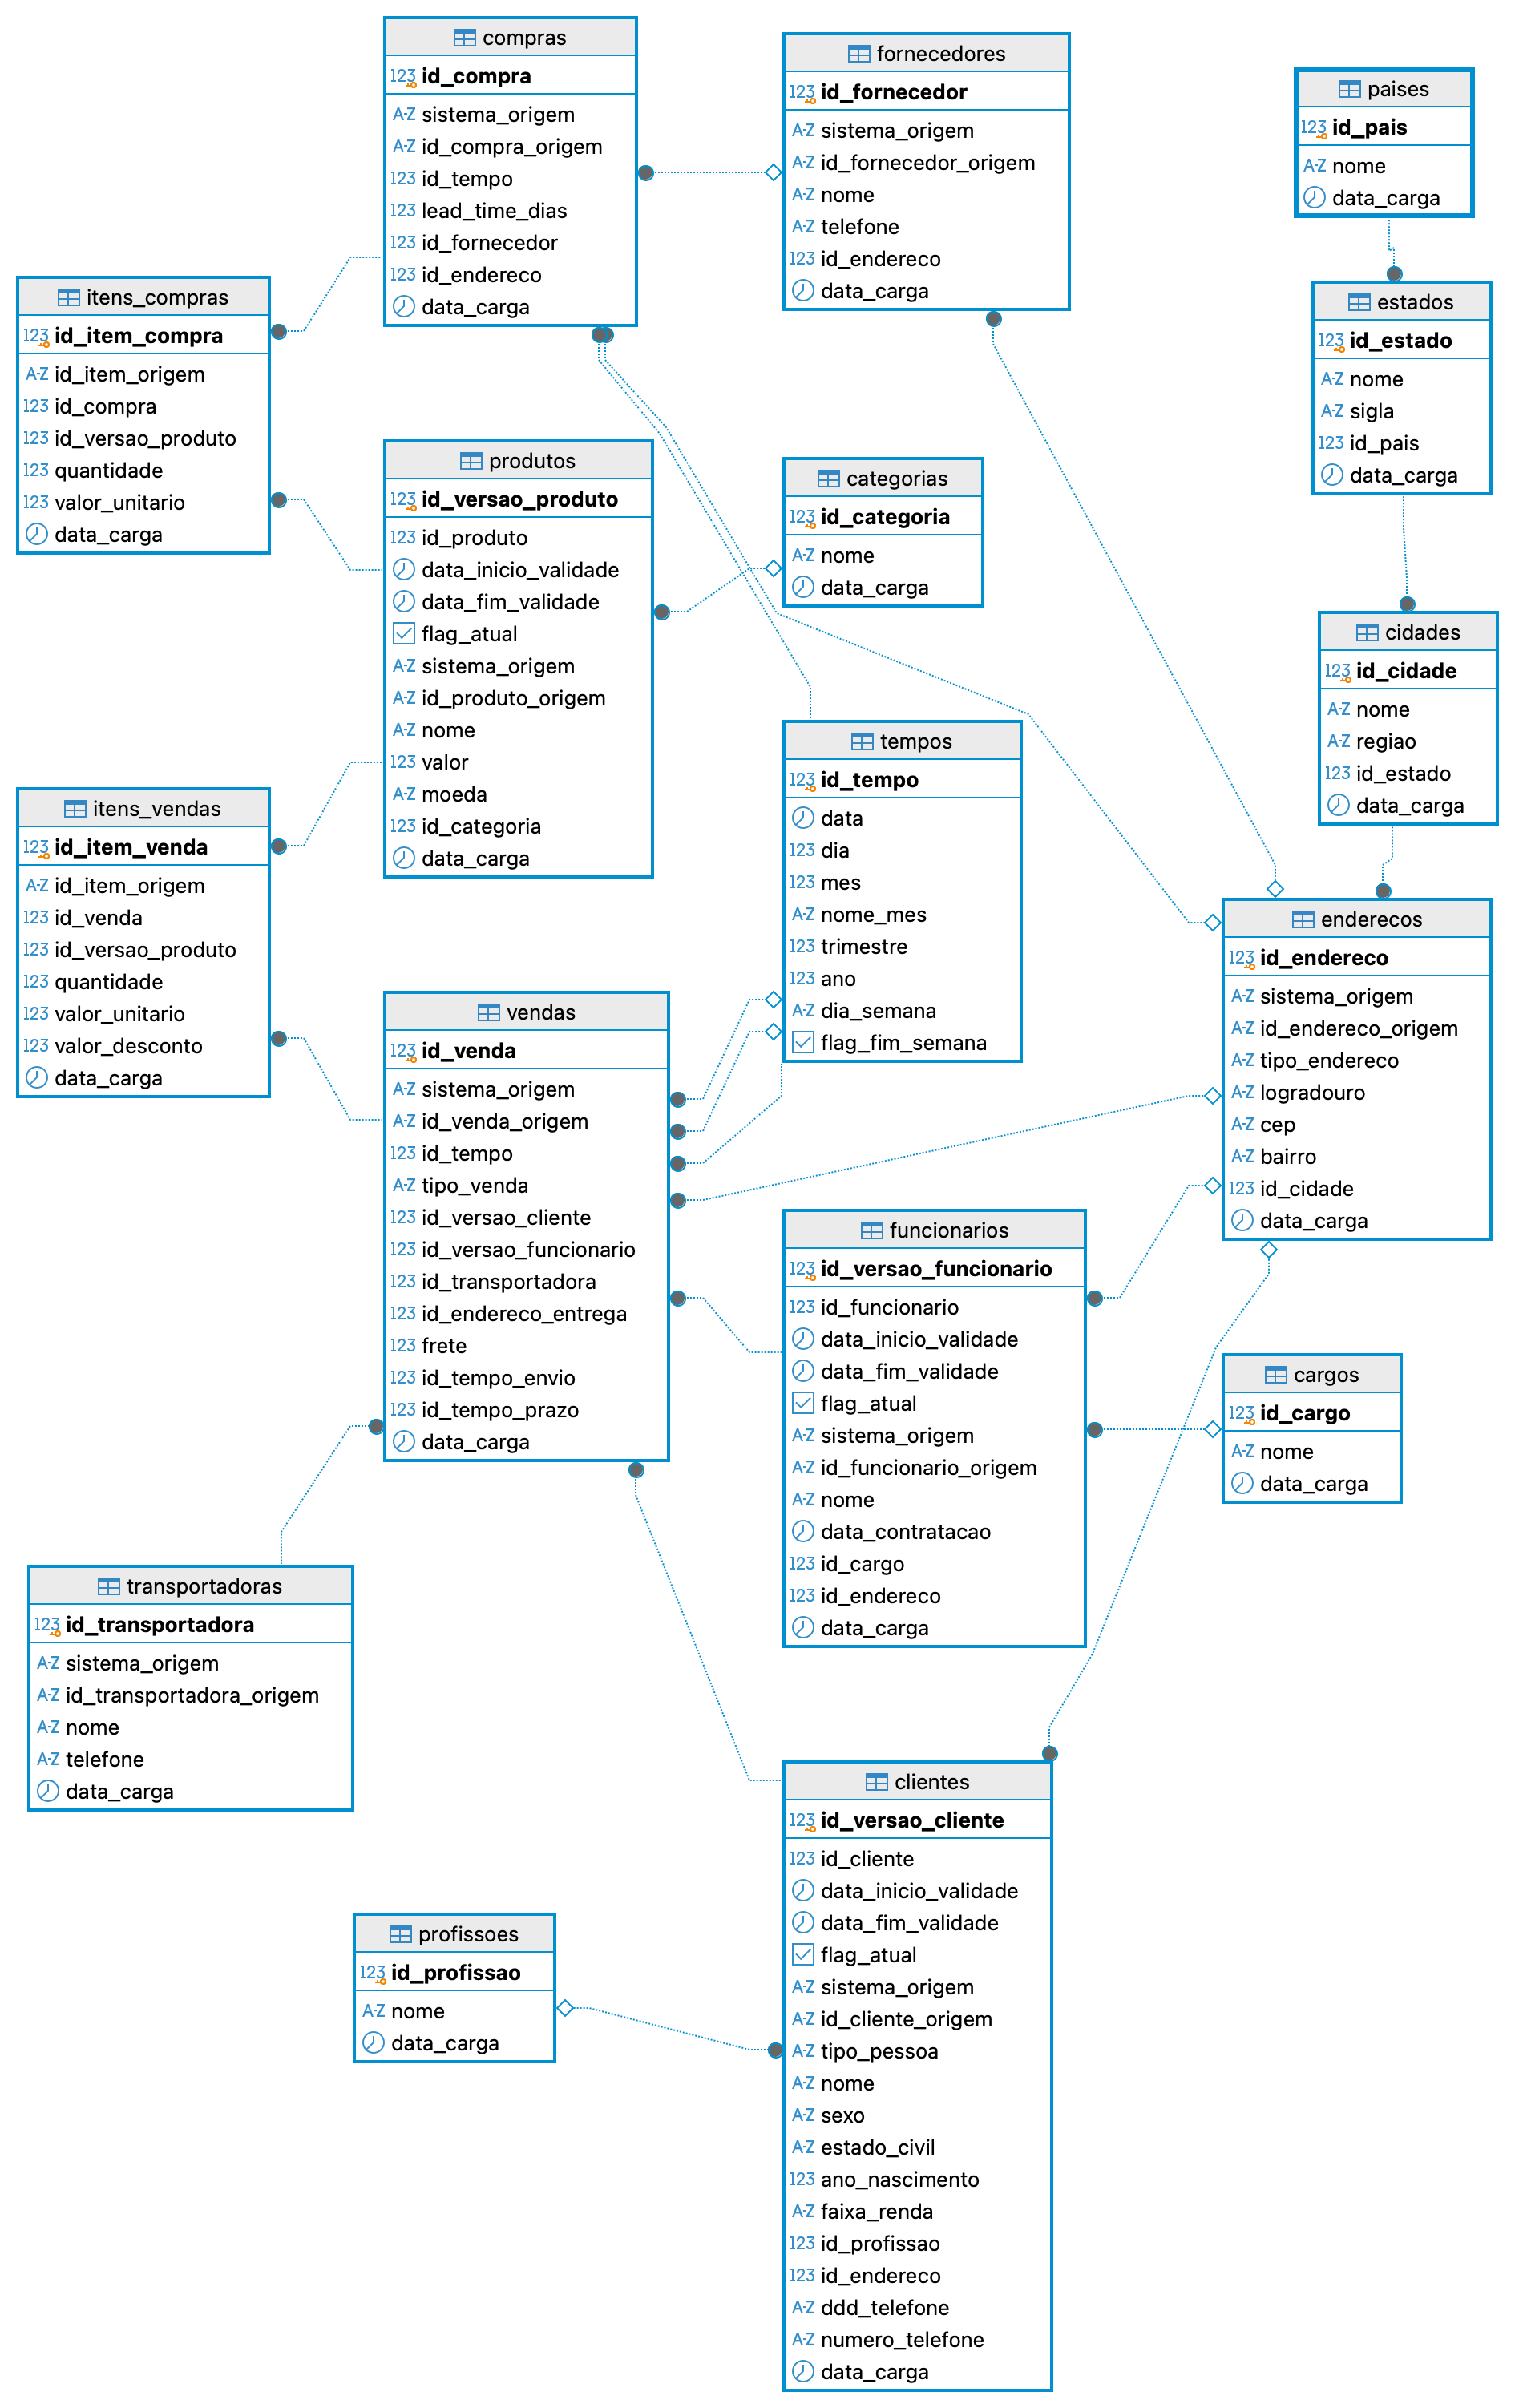
\includegraphics[width=0.8\textwidth]{./fig/dw_corporativo.png}
  \caption{Diagrama entidade-relacionamento do DW Organizacional}
  \label{fig:dw-corporativo}
  \fontefig{Elaborada pelo autor.}
\end{figure}

\begin{itemize}
    \item \textbf{Integração}: chave corporativa própria por sequência (ex.: \texttt{corporativo.seq\_clientes}) + \texttt{sistema\_origem}/id original para rastreabilidade;
    \item \textbf{Historicidade (SCD2)}: quando um atributo de cliente, funcionário ou produto muda (por exemplo, um cliente muda de faixa de renda), a linha antiga não é alterada; uma nova linha é inserida com a nova versão, e a antiga fica marcada como encerrada. Assim, o histórico completo fica preservado, e não só o valor mais recente;
    \item \textbf{Granularidade}: \texttt{vendas}/\texttt{itens\_vendas} e \texttt{compras}/\texttt{itens\_compras} têm grão de item;
    \item \textbf{Dados externos}: moeda fixa (\texttt{'BRL'}), \texttt{sistema\_origem} e membro sentinela \texttt{-1} ("Não aplicável") são atribuídos pelo ETL, documentados no catálogo de metadados (\autoref{cap:etl-bi}) como "Regras de Negócio do ETL".
\end{itemize}

DDL completo no \autoref{apend:ddl-dw}.
